\begin{frame}[fragile]{AST}
    \begin{itemize}
        \item \emph{Apstraktno sintaksno stablo} je stablo reprezentacije apstraktne sintaksne strukture koda pisanog u nekom programskom jeziku
        \item Svaki \v{c}vor drveta odgovara nekom konstruktu koda
    \end{itemize}
\begin{figure}[!h]
\centering
\begin{tabular}{ p{4.5cm} p{4.5cm} }
\begin{lstlisting}
while (x < 20)
    x = x + y * 2;
\end{lstlisting}
\end{tabular}
\end{figure}
\end{frame}


\begin{frame}[fragile]{AST}
\begin{figure}[!h]
\centering
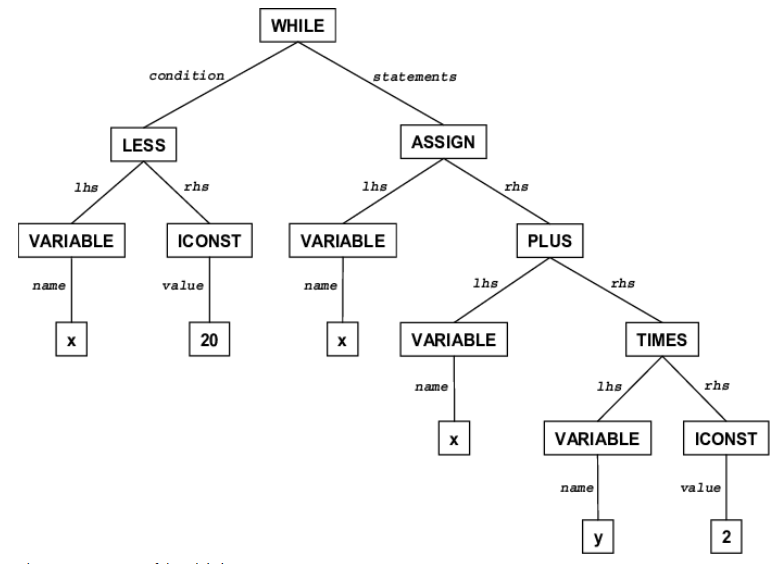
\includegraphics[scale=0.45]{../paper/res/WhileAST.PNG}
\end{figure}
\end{frame}
